\documentclass[12pt]{article}
\usepackage{changepage,soul,graphicx,graphbox,stoversymb}%,afterpage}
\usepackage[left=0.5in,right=0.5in,bottom=1in,top=0.75in]{geometry}%,showframe=true
\everymath{\displaystyle}

\usepackage[many]{tcolorbox}
\usepackage[inline]{enumitem}
\usepackage{amsmath,amsthm}
	\theoremstyle{definition}
	\newtheorem{defn}{Definition}
	
	\newtheoremstyle{underl}{4.5mm}{4.5mm}{}{}{}{\textnormal{.}}{ }{\underline{\thmname{#1}}}
	\theoremstyle{underl}
	\newtheorem*{ex}{Ex}

\thispagestyle{empty}

\newcommand{\capt}[1]{\begin{adjustwidth}{0.5in}{0.5in}\centering\small\textit{#1}\end{adjustwidth}}
\newcommand{\notebox}[2]
{\begin{tcolorbox}[
		enhanced,
		colback=white,
		colframe=black,
		boxrule=0.5pt,
		arc=0pt,
		top=3mm,
		bottom=3mm, 
		grow to left by=-0.5in,
		grow to right by=-0.5in
	]
	\noindent\textbf{#1}\\
	{#2}
\end{tcolorbox}}
\newcommand{\hintbf}[1]{\textbf{Hint}: #1}

\begin{document}
	\section*{\centering Exam 1 Preview}
	Below are some sample questions that you should be able to answer from chapter 2; don't be surprised if several of these end up looking like exam questions.
	
	\begin{enumerate}
		\item The following questions are about the ODE 
		$$\dydx=-3\left(1-\frac{y}{5}\right)\left(1-\frac{y}{9}\right) y.$$
		\begin{enumerate}[itemsep=0.25in, topsep=3mm, leftmargin=0.25in, rightmargin=0.25in]
			\item Find the equilibrium solutions of this ODE.
			\item Classify each of the equilibrium solutions as asymptotically stable, asymptotically unstable, or neither. \hintbf{Do not assume that $y>0$!}
			\item Assuming that $y(0)=2$, find $\lim_{x\to\infty}y(x)$. \textbf{Do not solve the ODE!}
			\item Which of the following phase lines correspond to this ODE?
				\begin{enumerate}[label=\roman*), topsep=6mm, itemsep=0.25in]
					\item 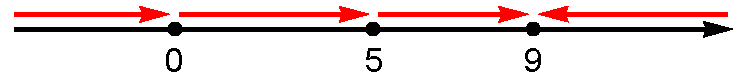
\includegraphics[align=c,scale=0.75]{phase2}
					\item 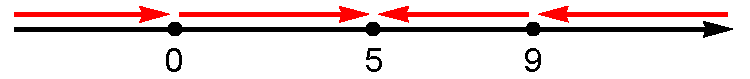
\includegraphics[align=c,scale=0.75]{phase3}
					\item 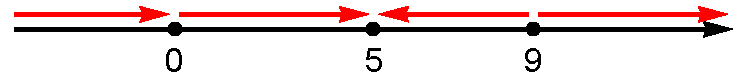
\includegraphics[align=c,scale=0.75]{phase4}
					\item 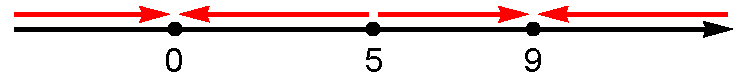
\includegraphics[align=c,scale=0.75]{phase1}
					\item 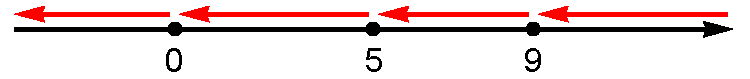
\includegraphics[align=c,scale=0.75]{phase6}
					\item 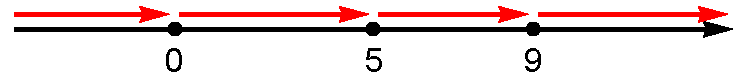
\includegraphics[align=c,scale=0.75]{phase5}
					\item None of the above
				\end{enumerate}
			\item Sketch the solutions to this ODE using the qualitative methods discussed in class. \textbf{Do not solve the ODE!}
			\item \textbf{True or False:} This ODE is linear.
			\item Which of the following slope fields correspond to this ODE?
			\vspace{6mm}
			\begin{adjustwidth}{-2in}{-1.5in}
				\begin{center}
					{
						\begin{tabular}{ccc}
							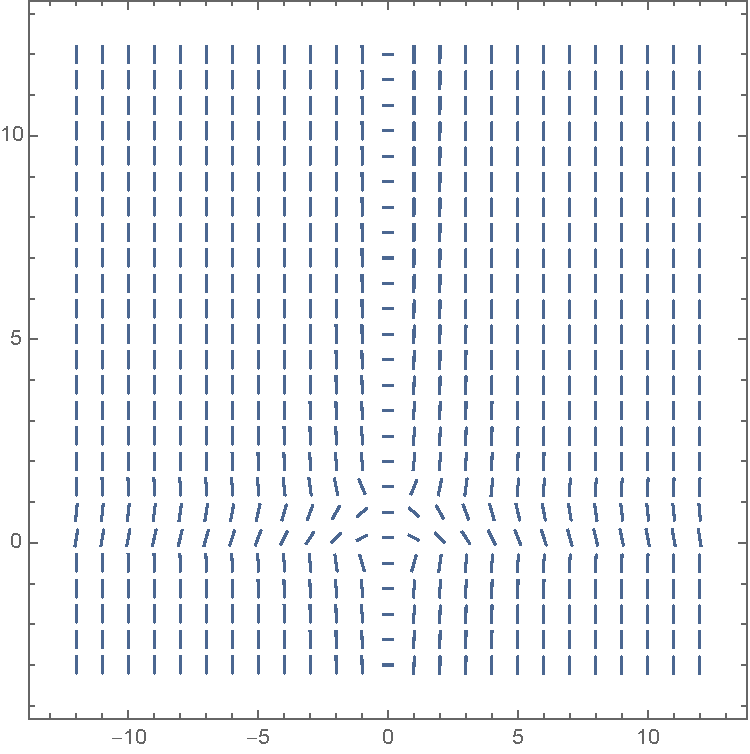
\includegraphics[width=3.25in,height=3.25in]{slopes2}& &
							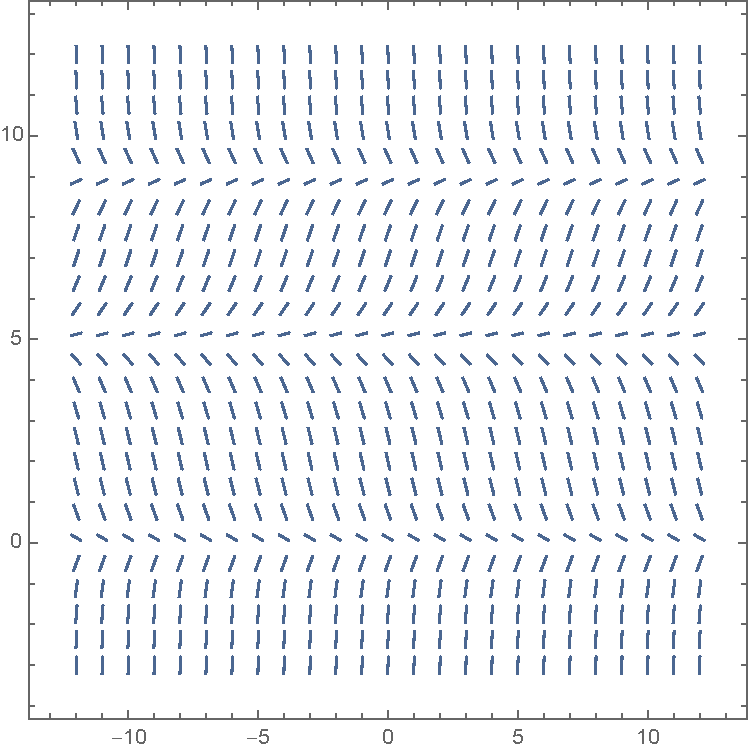
\includegraphics[width=3.25in,height=3.25in]{slopes1} \\
							\Large{(i)} &  & \Large{(ii)}\\[9mm]
							
							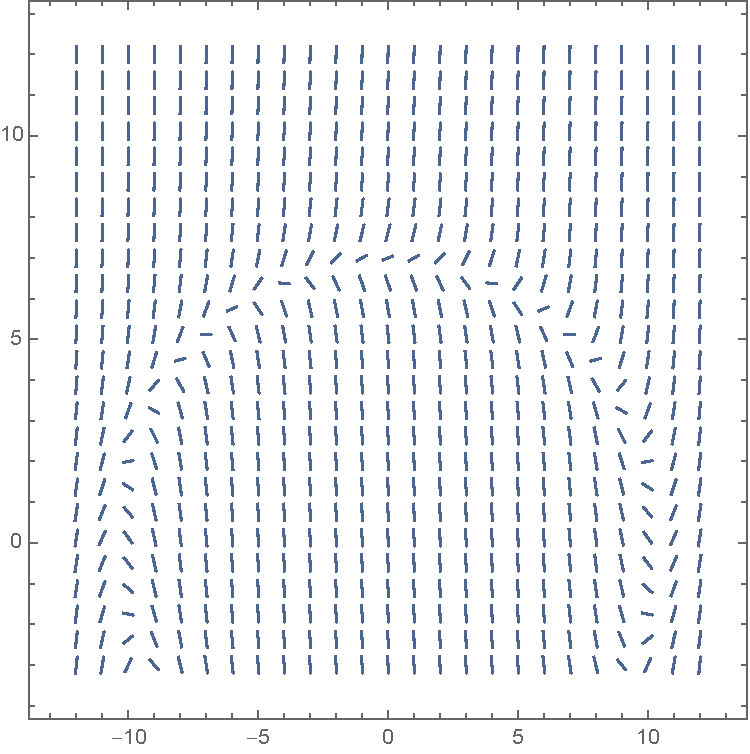
\includegraphics[width=3.25in,height=3.25in]{slopes4} & &
							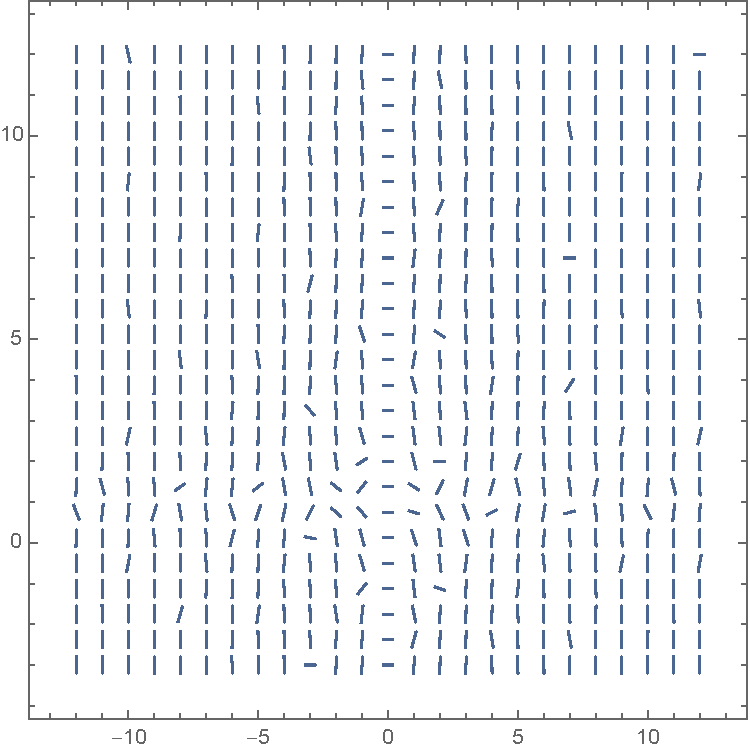
\includegraphics[width=3.25in,height=3.25in]{slopes3} \\
							\Large{(iii)} & & \Large{(iv)}\\
						\end{tabular}
					}%
				\end{center}
			\end{adjustwidth}
			\item Find the general solution of this ODE. \hintbf{Expect to use partial fractions!}
			\item Solve the IVP $\dydx=-3\left(1-\frac{y}{5}\right)\left(1-\frac{y}{9}\right) y$, $y(-1)=\pi$.
		\end{enumerate}
	\end{enumerate}
\end{document}